\subsection{RF Results}

We apply crossvalidation in the number of trees and depth of the forests for the 23 EoS, fixing the information gain criteria to \texttt{entropy}. We also save the second best option for comparison, and save both forests for each EoS in order to compare the file size. As the goal is to provide a model that can run in a low latency pipeline the amount of memory it can take is limited, even more when there will be 23 different model for the EoS generalization.



To simplify the model and according to the results of crossvalidation, we train the final forests for all EoS with 50 trees and 15 maximum depth. In figure \ref{fig:RF_roc} we show the ROC curves for all models to give an idea of the performance. Notice that HasREM performs better than HasNS. 
\begin{figure}
\centering
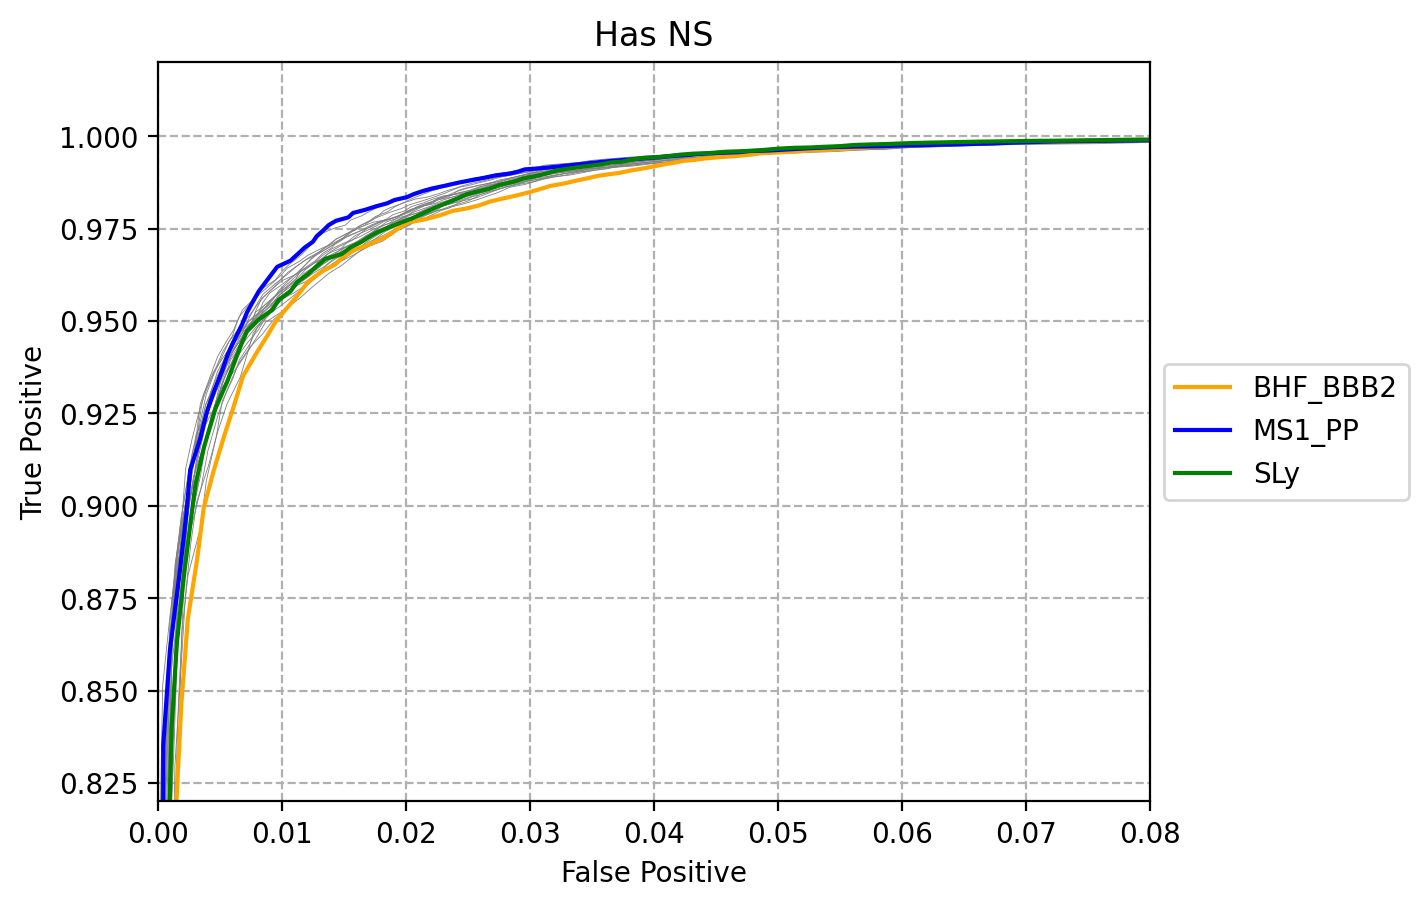
\includegraphics[width=0.45\textwidth]{/figs/HasNS_roc}
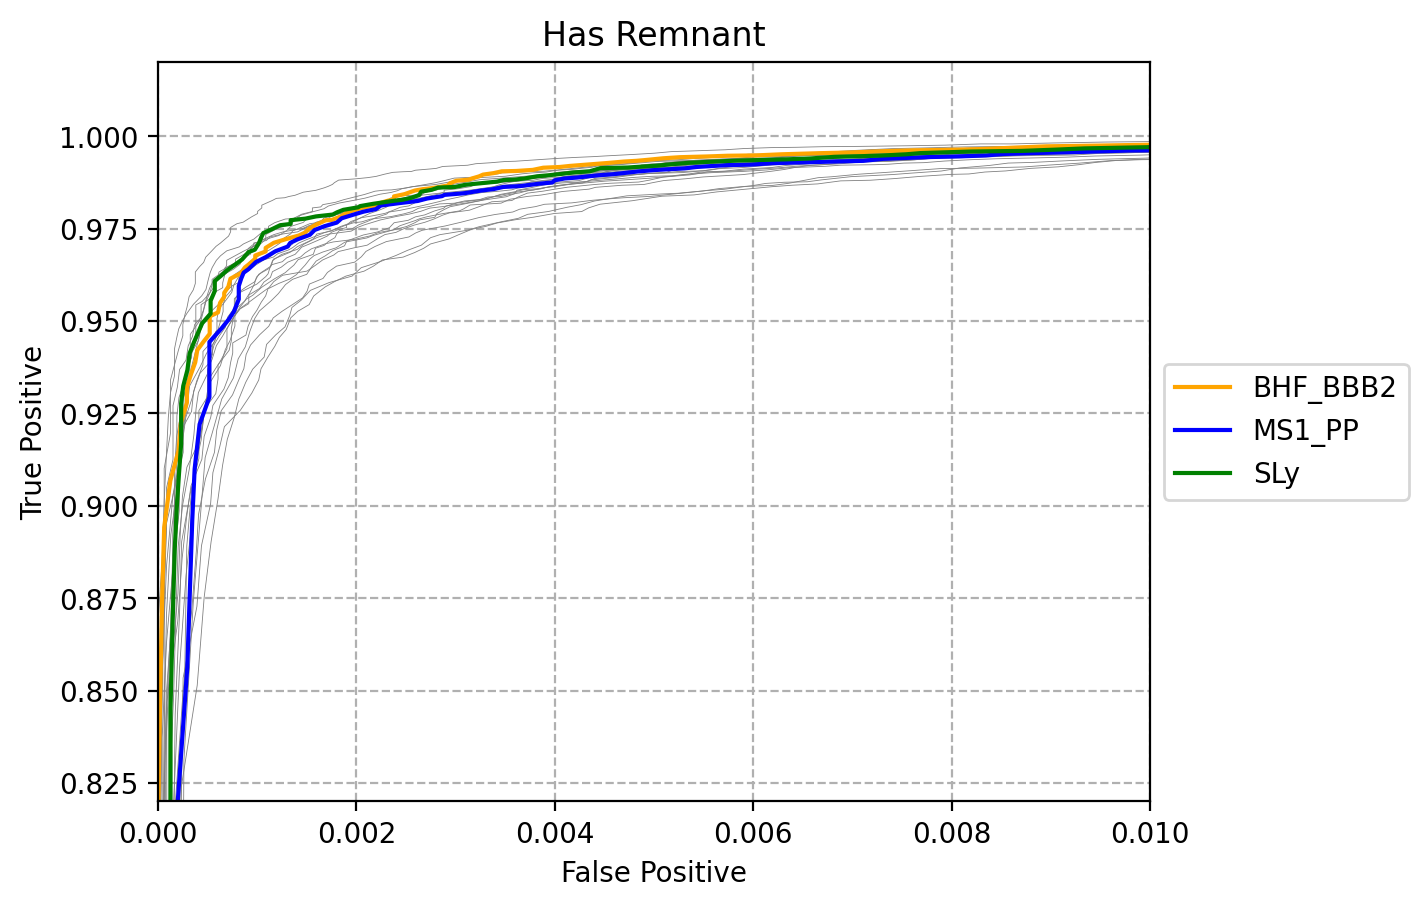
\includegraphics[width=0.45\textwidth]{/figs/HasREM_roc}
\caption{\label{fig:RF_roc} ROC curves RF}
\end{figure}




